\documentclass{ctexart}
%\usepackage{xeCJK}
%\usepackage[T1]{fontenc}
%\usepackage{mathptmx}
\usepackage{amsmath,amssymb,amsthm,color,mathrsfs}
\usepackage{enumitem,anysize}
\usepackage{geometry}
\usepackage{lipsum}
\usepackage{bbm}
\usepackage{tikz}
\usepackage{hyperref}
\hypersetup{
	hypertex=true,
	colorlinks=true,
	linkcolor=red,
	filecolor=blue,      
	urlcolor=blue,
	citecolor=cyan,
}

\geometry{a4paper,left=2.5cm,right=2.5cm,top=2.5cm,bottom=2.5cm}

\def\<{\langle}
\def\>{\rangle}
\edef\lim{\displaystyle\lim}
\def\email#1{\href{mailto:#1}{\texttt{#1}}}

\newtheorem{problem}{\textbf{Problem}}
\renewcommand\theproblem{\textbf{\Roman{problem}}}
\newenvironment{solution}{\begin{proof}[\textbf{Solution}]}{\end{proof}}

\renewcommand\phi{\varphi}
\renewcommand{\(}{\left(}
\renewcommand{\)}{\right)}
\renewcommand{\d}{\mathrm{d}}
\newcommand{\supp}{\mathrm{supp}}
\newcommand{\N}{\mathbb{N}}
\newcommand{\E}{\mathbb{E}}
\newcommand{\calU}{\mathcal{U}}
\newcommand{\R}{\mathbb{R}}
\newcommand{\shi}{\mathbbm{1}}
\renewcommand{\epsilon}{\varepsilon}
%\renewcommand{\empty}{\emptyset}





\newcommand{\minus}{\mathbin{\backslash}}

\newtheorem{lemma}{Lemma}
\newtheorem{cora}{Corallary}




\pagestyle{empty}
\title{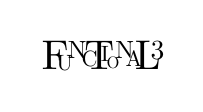
\begin{tikzpicture}[baseline]%
\node [scale=1.5] at (0.0em,0.0em) {F};%
\node [scale=0.8] at (0.35em,-0.25em) {U};%
\node [scale=0.9] at (0.8em,0.2em) {N};%
\node [scale=0.8] at (1.25em,-0.1em) {C};%
\node [scale=1.5] at (1.6em,0.0em) {T};%
\node [scale=0.8] at (1.8em,0.05em) {I};%
\node [scale=0.6] at (2.1em,-0.25em) {O};%
\node [scale=0.9] at (2.52em,0.2em) {N};%
\node [scale=0.8] at (2.85em,-0.1em) {A};%
\node [scale=1.5] at (3.35em,0.0em) {L};%
\node [scale=1] at (3.7em,0.18em) {3};%
\end{tikzpicture}}
\author{王胤雅\\
SID:201911010205\\
\email{201911010205@mail.bnu.edu.cn}}

\iffalse
1 
2 
\fi

\begin{document}
\large
\maketitle
\begin{problem}
	设 $F$ 是只有有限项不为零的实数列全体, 在 $F$ 上引入距离
	$$
	\rho(x, y)=\sup _{k \geq 1}\left|\xi_k-\eta_k\right|, \quad \forall x=\left(\xi_k\right)_{k \geq 1}, y=\left(\zeta_k\right)_{k \geq 1} \in F .
	$$
	求证 $(F, \rho)$ 不完备. 并求其完备化空间.
\end{problem}
\begin{proof}
	\begin{itemize}
		\item $(F,\rho)$ is not complete:\\
		$\{x^{(n)}\in F:x^{(n)}_k=\frac{1}{k}\shi_{k\leq n},n\in\N_+, k\in\N_+\}, x:=\{\frac{1}{n}\}_{n=1}^{\infty}$. Since $\forall x^{(n)},x^{(m)}\in F, n\leq m$, $\rho(x^{(n)},x^{(m)})=\sup_{k\geq 1}|x^{(n)}_k-x^{(m)}_k|=\frac{1}{n+1}\to 0$, when $n,m\to \infty$, then $\{x^{(n)}\}_{n=1}^{\infty}$ is a cauchy sequence on $(F,\rho)$. However, $\rho(x^{(n)},x)=\frac{1}{n+1}\to 0, n\to \infty$, by the uniqueness of limit, $\lim_{n\to\infty}x^{(n)}=x\notin F$.
		\item Consider $(E,\rho)$ where $E:=\{\{x_n\}_{n=1}^{\infty}: x_n\in\R\}$, which is a complete metric  space. 
		It is obvious that $(E,\rho)\supset (F,\rho)$. 
		We need to find the closer of $F$ in $E$. 
		$\forall \epsilon>0, x\in F$, $B(x,\epsilon):=\{y\in E: \rho(y,x)<\epsilon\}$, 
		let $m:=\sup\{k:x_k\neq 0\}$,$\forall y\in B(x,\epsilon),$
		 $\rho(x,y)=\sup\{\max_{1\leq k\leq m}|x_k-y_k|,\sup_{k>m}|y_k|\}<\epsilon$, 
		 then $\sup_{k>m}|y_k|<\epsilon$, 
		 so $\lim_{k\to\infty} y_k=0$, 
		 as $\epsilon\to 0$.\\
		\item \begin{itemize}
			\item $H:=\{\{x_{n}\}_{n=1}^{\infty}\in E:\lim_{k\to \infty} x_k=0\}$ is complete. 
			We need to proof $H$ is closed in $E$. 
			$\forall x^{(n)}\in H, n\in\N_+$, 
			and $x^{(n)}\to x:=\{x_n\}_{n=1}^{\infty}$, 
			then $\forall \epsilon>0$, $\exists N$, 
			$\forall n\geq N$, 
			$\sup_{k\geq 1}|x^{(n)}_k-x_k|<\epsilon/3$, 
			$\exists G$, $\forall k,j\geq G$, $|x^{(N)}_k-x^{(N)}_j|<\epsilon/3$,
			$\exists M$, $\forall j\geq M$, satisfies $|x^{(N)}_j|\leq\epsilon/3$. 
			Therefore $L:=\max\{G,M\},\forall k,j\geq L$, $|x_k|\leq|x_k-x^{(N)}_k|+|x^{(N)}_k-x^{(N)}_j|+|x^{(N)}_j|<\epsilon$. 
			Thus, $x\in H$.
			\item  Consider $\phi:F\to H$ which is an embedding map. 
			$\forall x\in H$, then $y_k:=\{x_k\shi_{k\leq n}\}\in F$. And $\rho(y_k,x)=\sup_{i\geq k+1}|x_{i}|\to 0$ 
			means $F$ is dense in $H$. 
		\end{itemize}
		
 	\end{itemize}
	
\end{proof}
\begin{problem}
	设 $(X, \rho)$ 完备, $\left\{F_n\right\}$ 是 $X$ 内的单调下降非空闭集序列,即
$$
F_1 \supset F_2 \supset \cdots \supset F_n \supset \cdots, F_n \neq \varnothing
$$
且 $F_n$ 的直径 $d_n=d\left(F_n\right) \rightarrow 0$.
证明: $\bigcap_{n \geq 1} F_n \neq \varnothing$. 如果没有条件 $d_n \rightarrow 0$, 结论成立吗?
如果 $X$ 为列紧空间时, 关于直径的条件是否还需要?
\end{problem}
\begin{proof}
	\begin{enumerate}
		\item 
		\iffalse  If $\exists N, \forall n\geq N, F_n=F_{n+1}$, then $\cap_{n=1}^{\infty} F_n= F_N\neq \emptyset$.
		Assume $\forall N$, $\exists n >N$ s.t. $F_n\minus F_{n+1}\neq \emptyset$.\fi Let $x_1\in F_1$, $x_{k+1}\in F_{k+1}\minus F_{k}$ if $F_{k+1}\minus F_{k}\neq\emptyset$, otherwise $x_{k+1}=x_k$, if $F_{k+1}\minus F_{k}=\emptyset$. Consider $\{x_n\}_{n=1}^{\infty}$. $\forall \epsilon>0$, $\exists N$, $\forall n>m \geq N$, $\rho(x_n,x_m)\leq d_m<\epsilon$. So $\{x_n\}_{n=1}^{\infty}$ is a Cauchy sequence. Since $(x,\rho)$ is complete, $x=\lim_{n\to\infty}x_n\in X$. Besides, $\forall n$, $F_n$ is close, so $\{x_k\}_{k\geq n}\in F_n$, so $x\in F_n$. Then $x\in\cap_{n=1}^{\infty} F_n$. 
\item $(X,\rho)=(\R,\rho)$, where $\rho(x,y):=|x-y|$, $F_n:=[n,\infty)$, $\cap_{n=1}^{\infty}F_n=\emptyset$. Another example, $(\R,\rho)$, where $\rho(x,y)=1,x\neq y,\rho(x,y)=0,x=y$. $(\R,\rho)$ is complete, let $F_1:=\{x_1,\cdots, x_n,\cdots \}\subset \R: |F_1|=\aleph_0$, $F_{k+1}=F_k\minus\{x_k\}$, $\cap_{k=1}^n F_k=\emptyset$
\item Unnecessary. Since $X$ is sequence compact and complete, $X$ is compact. If $B=\cap_{n\geq 1}F_n=\emptyset$, then $\exists F_n$, $F_n\cap B=\emptyset$, then $\forall x\in F_n$, $\exists u_x: x\in u_x\subset X$ is open, and $\exists F_x\in\{F_n\}$ satisfies $u_x\cap F_x=\empty$. Let $\calU:=\{u_x:x\in F_n\}$, which is an open covery of $F_n$. Since $X$ is compact, $F_n$ is close in $X$, then $F_n$ is compact. So, $\exists \{u_{x_1},\cdots, u_{x_n}\}\subset \calU$ is a finite open covery of $F_n$, and $u_{x_k}\cap F_{x_k}=\emptyset$, thus $\emptyset=\cup_{k=1}^n(u_{x_k}\cap F_{x_k})\supset \cup_{k=1}^n u_{x_k}\cap(\cap_{k=1}^n F_{x_k})\supset F_n\cap(\cap_{k=1}^{n} F_{x_k})=F_m\neq\emptyset$, where $m=\min\{n,x_1,\cdots x_n\}$, contraction!
\end{enumerate}
\end{proof}


\end{document}